\documentclass[border=10pt]{standalone}

\usepackage{tikz}
\usepackage{tikzsymbols}
\usetikzlibrary{calc,patterns,shapes.geometric}

\def\centerarc[#1](#2)(#3:#4:#5){\draw[#1] ($(#2)+({#5*cos(#3)},{#5*sin(#3)})$) arc (#3:#4:#5);}

\begin{document}
	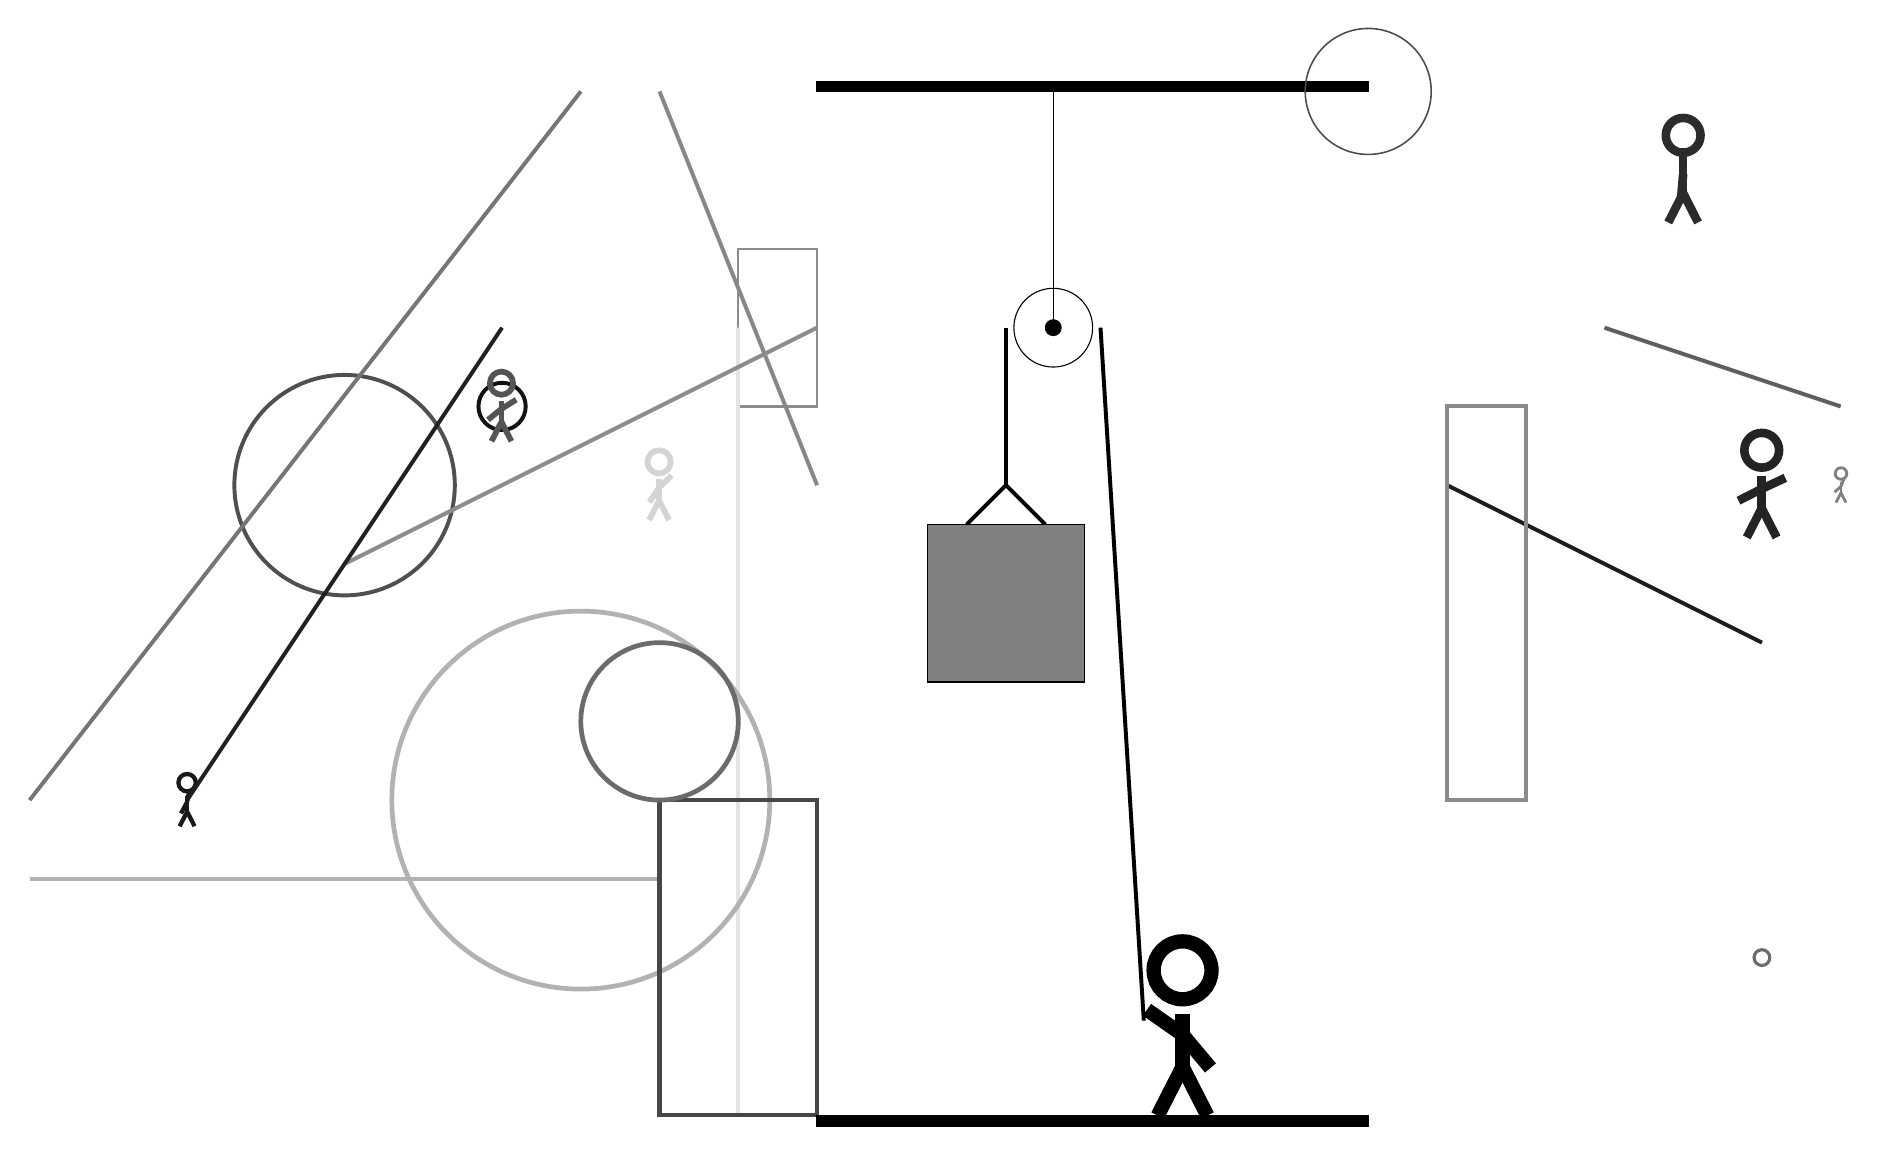
\begin{tikzpicture}
		%%%%% START %%%%%
		
		\draw[fill=black] (-2, 10) rectangle (5, 10.125);
		
		\draw (1, 7) circle (0.5);
		\draw[fill=black] (1, 7) circle (0.1);
		\draw (1, 10) -- (1, 7);
		
		\draw[line width=0.5mm] (-0.1, 4.5) -- (0.4, 5.0) -- (0.9, 4.5);
		\draw[fill=black!50] (-0.6, 4.5) rectangle (1.4, 2.5);
		
		\draw[line width=0.5mm] (0.4, 7) -- (0.4, 5.0);
		\centerarc[line width=0.5mm](1, 7)(0:180:0.6);
		\draw[line width=0.5mm](1.6, 7) -- (2.15, -1.8);
		
		\node at (2.6, -1.9) {\Strichmaxerl[10][-35][-50]};
		
		\draw[line width=0.3mm, color=black!45] (-3, 8) rectangle (-2, 6);
		
		\draw[line width=0.5mm, color=black!89](10, 3) -- (6, 5);
		\draw [line width=0.5mm, color=black!93](-6, 6) circle (0.3);
		\draw [line width=0.5mm, color=black!69](-8, 5) circle (1.4);
		\draw[line width=0.5mm, color=black!30](-4, 0) -- (-12, 0);
		\draw[line width=0.5mm, color=black!47](-2, 5) -- (-4, 10);
		
		\node[line width=0.2mm, color=black!17] at (-4, 5) {\Strichmaxerl[4][56][44]};
		\draw[line width=0.5mm, color=black!11] (-3, 7) rectangle (-3, -3);
		\node[line width=0.5mm, color=black!90] at (-10, 1) {\Strichmaxerl[3][62][79]};
		\draw [line width=0.2mm, color=black!70](5, 10) circle (0.8);
		\node[line width=0.7mm, color=black!83] at (9, 9) {\Strichmaxerl[6][85][90]};
		\draw[line width=0.5mm, color=black!54](-5, 10) -- (-12, 1);
		\draw [line width=0.6mm, color=black!30](-5, 1) circle (2.4);
		\draw [line width=0.4mm, color=black!58](10, -1) circle (0.1);
		\node[line width=0.2mm, color=black!86] at (10, 5) {\Strichmaxerl[6][27][25]};
		\draw[line width=0.5mm, color=black!45](-2, 7) -- (-8, 4);
		\draw[line width=0.5mm, color=black!63](8, 7) -- (11, 6);
		\draw[line width=0.5mm, color=black!87](-6, 7) -- (-10, 1);
		\draw[line width=0.6mm, color=black!72] (-4, 1) rectangle (-2, -3);
		
		\draw[line width=0.5mm, color=black!46] (7, 1) rectangle (6, 6);
		\node[line width=0.7mm, color=black!50] at (11, 5) {\Strichmaxerl[2][42][69]};
		
		\node[line width=0.2mm, color=black!67] at (-6, 6) {\Strichmaxerl[4][39][32]};
		
		\draw [line width=0.6mm, color=black!58](-4, 2) circle (1.0);
		
		\draw[fill=black] (-2, -3) rectangle (5, -3.15);
		
		%%%%% END %%%%%
	\end{tikzpicture}
\end{document}